\documentclass[border=4pt]{standalone}
% Preámbulo común de las figuras. Cada figura es un documento standalone
% que se compila a SVG con scripts/build_figures.sh
\usepackage[utf8]{inputenc}
\usepackage{amsmath}
\usepackage{tikz}
\usepackage[american, siunitx]{circuitikz}
\usetikzlibrary{arrows.meta,calc,decorations.pathmorphing,patterns}
\tikzset{
  >={Stealth[length=2.2mm]},
  eje/.style={->, thin},
  hilo/.style={thick},
}
% Paleta común: tonos medios legibles sobre fondo claro
\definecolor{azul}{RGB}{31,94,168}
\definecolor{rojo}{RGB}{192,57,43}
\definecolor{verde}{RGB}{39,128,73}
\definecolor{naranja}{RGB}{211,120,30}
\definecolor{morado}{RGB}{125,60,152}

\begin{document}
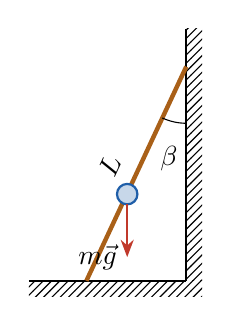
\begin{tikzpicture}[scale=1.0]
  % escalera de longitud L a 25 grados de la pared
  \fill[pattern=north east lines] (0,0) rectangle (0.2,3.2);
  \draw[thick] (0,0) -- (0,3.2);
  \fill[pattern=north east lines] (-2.0,-0.2) rectangle (0.2,0);
  \draw[thick] (-2.0,0) -- (0,0);
  \draw[line width=1.6pt, naranja!80!black] (-1.268,0) -- (0,2.719);
  \draw (0,2.0) arc (270:245:0.72); \node at (-0.22,1.55) {$\beta$};
  \node[rotate=65, above] at (-0.75,1.35) {$L$};
  \filldraw[draw=azul, fill=azul!25, thick] (-0.75,1.1) circle (0.13);
  \draw[->, thick, rojo] (-0.75,0.97) -- (-0.75,0.3) node[left, text=black]{$m\vec g$};
\end{tikzpicture}
\end{document}
